\documentclass{sig-alternate}
\usepackage{times}
\usepackage{epsfig}
\usepackage{graphicx}
\usepackage{amsmath}
\usepackage{amssymb}
\usepackage{epstopdf}
\usepackage[breaklinks=true,bookmarks=false]{hyperref}

\begin{document}

\title{Human Activity Recognition with Mobile Sensors}

\author{
Fridtjof Melle\\
Carnegie Mellon University\\
{\tt fmelle@andrew.cmu.edu}
}

\maketitle

%%%%%%%%% ABSTRACT
\begin{abstract}
   With the growing accessibility of accelerometers and movement measurement in our everyday lives largely introduced by smart phones we carry with us to all places the various ways of application are endless. A first step in making this an profitable tool for everyday use is to convert the measurements into something intelligent. Activity Recognition is a rising field where we seek to translate chains of time-series data provided by mobile sensors into specific activities. By intelligently analyzing this data this study seeks to determine what kind of activities are easily or more difficultly recognized using a simple and widely implemented posterior probability measuring classification algorithm.
   
\end{abstract}

%%%%%%%%% BODY TEXT
\section{Introduction}

\subsection{The Problem}
In the growing field of \textit{Human Activity Recognition} we find ourselves surrounded with the complex task of successfully and effectively translating endless variations of time-series recorded sensor data into meaningful resources. While we today profit from a large array of applications that to some extent recognizes human activity, most devices  limit themselves to certain specific types of activities in a given context such as sports or specific tasks. There is still a lot of work left to develop an all-understanding intelligence that can comprehend every type of activity induced into sensible information.

\subsection{The Solution}
In order to address this massive challenge, this research focuses on analyzing what kind of activities that are recognized most effectively, and what kind of activities require more consideration.

Through a simple standardization of an established and widely used dataset for \textit{Human Activity Recognition}, the study seeks to analyze the per-activity performance using the simplest and perhaps most widely used posterior probability classification method by looking at the various improvements that can be amended to it.

The validation of the results will be established using confusion matrices, precision, sensitivity and error analysis.

%=====================================================================

\section{Background}

\subsection{Dataset}
For the purpose of researching the proposed problem most efficiently, a well-tested and widely researched dataset was taken into consideration. The Skoda Mini Checkpoint dataset was originally created to investigate the use of ensemble classifiers in activity recognition and has been widely implemented over the past years\cite{Zappi08}. 

The dataset contains time-series data from a total of 10 USB sensor accelerometers equally placed and separately recorded on each arm over three hours resulting in about 700,000 data points each representing 33 ms visualized in Figure~\ref{fig:body_sensors}. Every sensor measures over three dimensions simultaneously collecting the effects of a total 10 manipulative gestures performed in a car maintenance scenario, as well as one null activity for reference. The resulting two fully labeled datasets for left and right arm form the basis for our study. 

\begin{figure}
\begin{center}
  \includegraphics[width=0.6\linewidth]{non_tech_imgs/Body_Sensors.png}
\end{center}
  \caption{Visualization of the mobile sensors placement.}
  \label{fig:body_sensors}
\end{figure}

\begin{table}[bp]
\centering
\caption{Mapping of activities to label values.}
\begin{tabular}{|l|l|}
\hline
\text{Activity}          				&\textbf{Label value} 	\\ \hline
\textbf{Null activity}  				& 32 		 			\\ \hline
\textbf{Write on notepad}	 			& 48		 			\\ \hline
\textbf{Open hood}  					& 49 					\\ \hline
\textbf{Close hood}				 		& 50 					\\ \hline
\textbf{Check Gaps on the front door} 	& 51 					\\ \hline
\textbf{Open left front door}	 		& 52 					\\ \hline
\textbf{Close left front door}			& 53 					\\ \hline
\textbf{Close both left doors}			& 54 					\\ \hline
\textbf{Check trunk gaps}				& 55 					\\ \hline
\textbf{Open and close trunk}			& 56 					\\ \hline
\textbf{Check steering wheel}			& 57 					\\ \hline
\end{tabular}
\label{tab:label_value}
\end{table}

\subsection{Sliding windows and Feature Extraction}
Classifying \textit{Human Activity Recognition} data is effectively translating time-series signal data into specifically performed sequences of gestures forming an activity.

The first step in establishing a dataset that can be injected into a statistical classifier is to evaluate the time-series data delicately. Inspired by previous approaches, an approach to capture local information for primitive-based AR by sliding windows with overflow was decided upon\cite{Huynh}.

With this configuration of the sliding windows, the feature vectors will be assembled by intelligently chosen features as established by previous approaches\cite{Zeng}.

%=====================================================================

\section{Overview}
The study is effectively divided into several main parts, each providing intelligent results towards the issue in question.

\subsection{Baseline Classification Performance}
In a first time we look closer at the baseline performance of our algorithm once applied most elegantly towards a preprocessed version of the original dataset. This approach serves in providing a ground understanding of how well the simplest evaluation of time-series data performs on a very specific set of a limited number of activities once trained on several repetitions of every activity.

\subsection{Combining The Data}
The original data provided by \textit{Skoda Mini Checkpoint} does as mentioned contain data separately measured from sensors equally spread and placed on both arms. While it is interesting to evaluate how various activities are recognized with different amounts of success by each arm individually, the study investigates how intelligently merging the two separate datasets improves the recognition. 

This will consequently provide understanding of how more doubling the amount of information or sensors for each measurement increases the general classification performance.

\subsection{Feature Selection}
When attempting to recognize various activities, different sensors have varying impact on different activities. In collaboration with another team working on the same dataset for \textit{Human Activity Recognition}, the research was enhanced by the possibility of measuring the effect of performing a more extensive feature selection with subsequent dimensionality reduction on the same set of data. 

Looking at the performance of this approach explores the space of improvement in extracting more features while intelligently keeping the ones that should improve the discrimination between the activities and discarding those that make them look more similar.

\subsection{Performance by Increasing Data Amount}
In a real-world application an implemented algorithm should not only perform very accurately, it will optimally also handle real-time received data from the sensors. To approach this with the provided dataset, the study will perform a brief assessment of the classification precision for percentage amounts of the original data ranging from 10\% to a maximum 100\%.

%=====================================================================

\begin{figure}[t]
\begin{center}
  \includegraphics[width=0.6\linewidth]{non_tech_imgs/knn_vis.png}
\end{center}
  \caption{A visualization of the nearest neighbors method.}
  \label{fig:knn_vis}
\end{figure}

\section{Preprocessing Time-Series Data}
As where the original \textit{Skoda Mini Checkpoint} comes with the measured data in both a converted calibrated acceleration measure and a raw ADC read-out format, the research focuses on looking at the simplest formulation in only implementing the raw acceleration data.

Although quite sophisticated approaches exist in evaluating the sliding window extraction method, this study focuses on mere simplicity for the purpose of developing a baseline and effectively uses a sliding window of 64 data points resulting each counting for about 2 seconds of measurement with 50\% overflow\cite{Zhang}.

Among the more complex feature extraction methods that has been considered by earlier approaches this study again focuses on simplicity. The two most primitive features was thus extracted from each sensor, in mean and standard deviation. This choice supports the goal of evaluating between other forms of improvement, extensive feature extraction.

As the original data is sorted chronologically according to the recording, a next step was needed to randomize the order before partitioning for training and testing. A complete randomization was performed using a simple method implemented in \textit{MATLAB}.

A last step in preparing the data was performing a 10 fold partitioning to prepare for cross-validation implementation in the classification step.

%=====================================================================

\begin{figure}[bp]
\begin{center}
\includegraphics[width=0.6\linewidth]{visual_results/evaluate_k_both_perf.jpg}
\end{center}
\caption{Precision evaluation for number of nearest neighbors.}
\label{fig:eval_k_both_perf}
\end{figure}

\section{Algorithm}
In the terms of developing the most simplistic classification algorithm, the \textit{k nearest neighbors} was found ideal. Amongst the various posterior probability measuring algorithms this algorithm makes no assumption of the data distribution and performing deterministic association on a adjustable local scope as depicted in Figure~\ref{fig:knn_vis}. This approach justifies its purpose of analyzing which activities that are likely to be misclassified. 

The algorithm is implemented by using \textit{MATLAB}'s publicly available libraries for \textit{KNN}, cross-validation and subsequent visualization and performance analysis. An effort was made to correctly make use of put together all the tools available to allocate time for analysis which is the key part of the study.

The code that went into the implementation of the proposed solution is visible at \url{http://tiny.cc/FMSDL14}.

\subsection{Configuring the KNN}
Once partitioned the \textit{KNN} effectively makes use of a 10-fold cross-validation for both determining its parameters and performing the general classification. In a total of ten iterations, it trains on nine of the partitions and tests on one. This allows us to predict on ever data point that is available to minimize the opportunity for over-fitting the parameter $k$ and maximizing the validity of the performance results.

\begin{figure}
\begin{center}
\includegraphics[width=0.6\linewidth]{visual_results/evaluate_k_both_loss_pred_error.jpg}
\end{center}
\caption{Error evaluation for number of nearest neighbors.}
\label{fig:eval_k_both_error}
\end{figure}

Evaluating the number of neighbors is a delicate process where several evaluations is taken into account, seeking a compromise between precision and error. Focusing primarily on minimizing the error rate of the classifier every dataset that was evaluated went through the same parameter validation process. With 11 total different classes the process looked at error and performance for $k$ ranging between one and ten voting neighbors, using a reduced dataset with the same 10-fold cross-validation scheme as in the classification.

The process is illustrated for the combined data set in Figure~\ref{fig:eval_k_both_perf} and Figure~\ref{fig:eval_k_both_error}, visualizing the precision and error rate for $k$ respectively. 

As is usual with this type of deterministic association, $k=1$ nearest neighbor is quite prone to overfitting and even excellent results for this value should be ignored. With quite few classes kind of graph output was typical for all the processed datasets. In this example the optimal number of nearest neighbors is easily observed, as both graphs has their most apparent extremity for $k=5$ which is consequently the optimal $k$ for this dataset of combined data from left and right arm. The results regarding all the datasets processed by the validation scheme is displayed in Table~\ref{tab:optimal_k}.

\begin{table}[t]
\centering
\caption{Validation results of optimal nearest neighbors.}
\begin{tabular}{|l|l|}
\hline
           			&\textbf{Optimal $k$} 	\\ \hline
\textbf{Left arm}  						& 3 		 				\\ \hline
\textbf{Right arm} 						& 3		 					\\ \hline
\textbf{Combined}  						& 5 						\\ \hline
\textbf{Right arm LDA processed} 		& 7 						\\ \hline
\textbf{Left arm LDA processed} 		& 7 						\\ \hline

\end{tabular}
\label{tab:optimal_k}
\end{table}

%=====================================================================

\section{Analysis}
\subsection{Baseline Classification Performance}
The basis of this study is to first evaluate what the most restrictive classification method can achieve in terms of each activity. The data provided being divided into two separate sets representing respectively the left and right arm the first iteration looks at the performance towards each of these and evaluates the immediate differences.

\subsubsection{Left arm evaluation}
Applying our algorithm to the left arm dataset yields the per-activity performance for the 10 sensors connected to the left arm only. The baseline precision landed at 92.03\%, with a sensitivity and effectively an error rate at respectively 92.02\% and 7.96\%. 

In order to evaluate the per-activity performance we can look closer at the confusion matrix visualized in Figure~\ref{fig:conf_left_surf} and further broken down in the table structure in Figure~\ref{fig:conf_left}.

We can observe a generally strong diagonal indicating the true positive rate, specifically peaking at activities 48 (Write on notepad), 55 (Check trunk gaps)  and 51 (Check gaps on the front door) performing as high as 97.97\% for Writing on notepad. The intuitive reason for this high performance is most naturally that these activities are individually quite different from all the others from a left-arm perspective. 

On the other side of the scale we find activities 49 (Open hood), 52 (Open left front door) and 53 (Close left door). The pair of opening and closing left front door is in particular confused heavily with each other with respectively 6.0\% and 7.1\% confusion, achieving 75.98\% and 81.43\%. Naturally these sequence of gestures are to some extent just the opposite one from the other, with only a handful of sensors measuring just the opposite value. With no weighting to any of the sensors in particular this is a natural consequence as the gesture for most sensors can be observed as just the same.

At 87.7\% the activity of opening the hood is also quite below average being confused with closing the hood at 6.99\%. While this is not the case visa-versa, the confusion might easily be tracked to that opening the hood is usually a right-hand activity. Finally the null activity is generally confused with all other activities intuitively being voted when a performed activity is not discriminant enough from doing nothing.

\begin{figure}[bp]
  \centering
  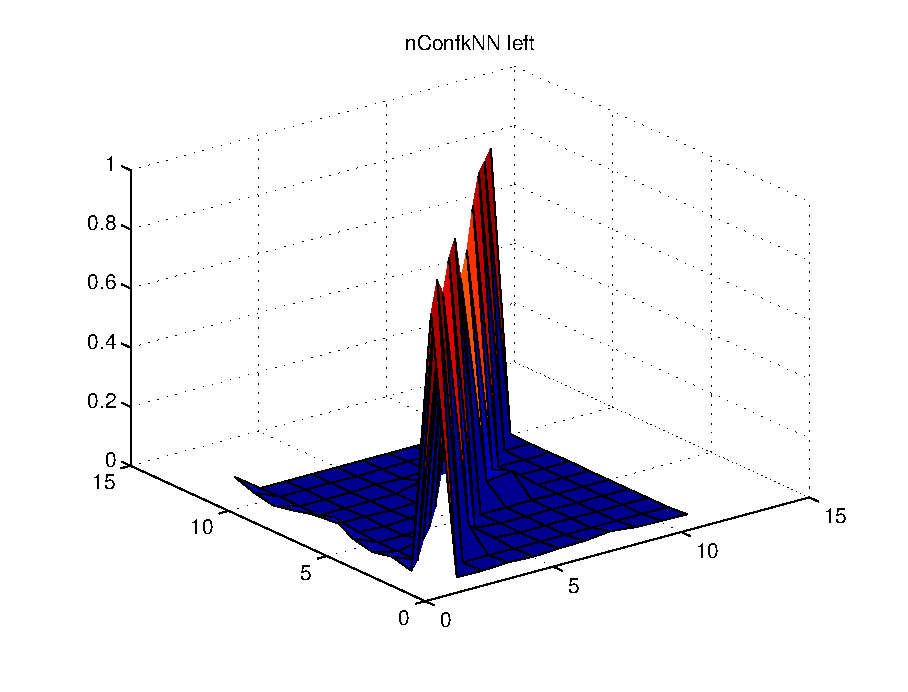
\includegraphics[scale=0.4]{./matlab_output/nConfkNN_left.eps}
  \caption{Visualization of the left arm confusion matrix.}
  \label{fig:conf_left_surf}
\end{figure}

\subsubsection{Right arm evaluation}
Performing the same evaluation on the right-arm dataset we achieve a similar, but although differing result. This baseline performance concluded at 90.95\% particularly with a 89.85\% sensitivity and effectively an error rate at 9.05\%.

Looking closer at the confusion matrix visualized in Figure~\ref{fig:conf_right_surf} and broken down in Figure~\ref{fig:conf_right} we can observe that the performance is generally of the same trends as the left-arm data. 

The best performance is for activities 48 (Write on notepad), 51 (Check gaps on front door), 54 (Close both left doors) and 56 (Open and close trunk) with writing on notepad equally peaking on 97.77\%. This be tracked to the fact that these are all heavily right-arm involving activities.

The statistically worst performers include the same activities as was found difficult by the left-arm dataset. The pairs of open vs. close hood (49 and 50) and open vs. close left door (52 and 53) are effectively the worst performers. More specifically opening and closing left door distinct themselves in performing well below the other activities at a striking 73.65\% and 70.61\% respectively, being confused at 15.35\% and 18.42\% with each other and 10.58\% and 10.97\% with the null activity.

\begin{figure}
  \centering
  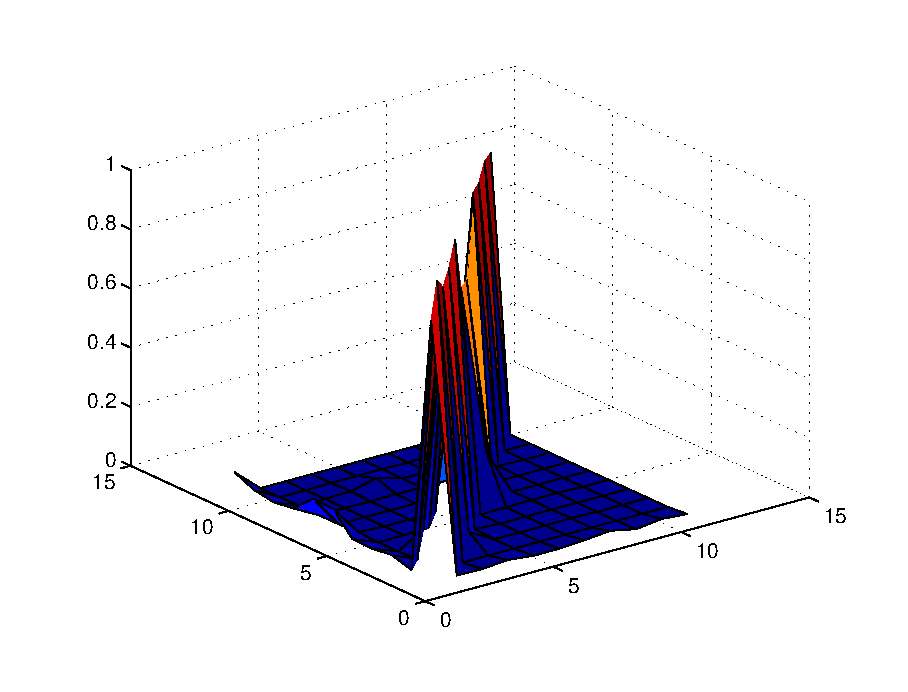
\includegraphics[scale=0.4]{./matlab_output/nConfkNN_right.eps}
  \caption{Visualization of the right arm confusion matrix.}
  \label{fig:conf_right_surf}
\end{figure}

\subsubsection{Comparative conclusions}
The general performance of both left and right arm data classification is depicted in Table~\ref{tab:comp_left_right}. While the precision simply represents our classification correctness, the recall rate is bound to the sensitivity of our classifier. Looking at every activity it represents the number of activities classified as a specific activity over the actual sum data points labeled for that activity. The F1 score is widely used to evaluate classification schemes for a compromise between sensitivity and precision.

\begin{equation}
F_1 score = 2 \frac{precision * recall}{precision + recall}
\end{equation}

The positive results tells depicted in the table tells of generally strong performance. Observing the diagonals of both confusion matrices for true positive we find values for most activities well into the 90th percentile, reflected in the $F_1 score$s ending at respectively 92.03\% and 90.40\%.

The baseline is specifically good at quite distinct activities as writing on the noted, confirming the intuitive conclusion that distinct activities are naturally easier to classify from each other.

\begin{table}[bp]
\centering
\caption{Validation results of optimal nearest neighbors.}
\begin{tabular}{|l|l|l|}
\hline
           							&\textbf{Left arm} 				&\textbf{Right arm}		\\ \hline
\textbf{Precision}  				& 92.04\% 		 				& 90.95\%					\\ \hline
\textbf{Error rate} 				& 7.96\%		 				& 9.05\%					\\ \hline
\textbf{Sensitivity}  				& 92.02\%		 				& 89.85\%					\\ \hline
\textbf{$F_{1}$ score}  			& 92.03\%		 				& 90.40\%					\\ \hline

\end{tabular}
\label{tab:comp_left_right}
\end{table}

The under-performance of the right-hand data towards the left-arm dataset can statistically be traced to activities open vs. close left door (52 and 53). This issue can further intuitively be traced to the idea that the left door of a vehicle is naturally handled with left hand, letting the right arm slide along the body. This fact explains the internal confusion as well as with the null activity.

An apparent issue with the division of the sensors between arms is when evaluating activities that are primarily connected to the other arm. The inclusion of a null activity although has it value in reducing the overall false positive rate. One would for a real-world application rather want an activity not to be registered than having the application always submitting to another category when in doubt. We can therefore conclude with that the confusion towards this activity is of less grave nature and be content with the general performance of about 90\%, specifically in this case when looking at a limited number of sensor focused at one body-part.

The right-arm dataset also looses some performance due to reduced sensitivity. Looking at the null activity classification for this data we can see a higher success, but at a cost of classifying about 10\% of both open and close left door as null activities. The reasons for this having been mentioned this effectively reduces the sensitivity further distancing the datasets from each other.

The effect of the visualizations depicted in Figure~\ref{fig:conf_left_surf} and Figure~\ref{fig:conf_right_surf} is that we can observe the general resemblance in classification success. This effectively predicts that combining the data will not solve any problems as the issues overlap, although it should improve the classification to some extent.

\subsection{Combining The Data}
The first step in looking at the combined data of measurements from all 20 accelerometers involves merging the provided data.

The key issue with this task is that the datasets are effectively of different number of measures with respectively 696,975 and 705,904 data points each. With no indication of reason to this phenomenon in the provided data-description there can be several reasons to this. With an equal sampling rate of period 33 ms each the problem can either be with the right arm having an additional sensor yielding 10\% more data or just the fact that right-arm tasks are generally more usual, which in all cases remains as mere speculations.

The assumption made for the merging to take place is that each activity is commenced simultaneously with both arms from a chronological aspect. This enables us to effectively assume that the first data point for each activity for one set should correspond to the first data point of the same activity in the other, discarding eventual supplementary data points for the other arm on a previous activity should they be in imbalance.

The approach leads us to reduce the total number of data points our final merged dataset contains 687,769 rows of data. The validation of this merging is effectively measured by its performance relative to the baseline.

Doubling the amount of sensors for each measure strategically placed on non-overlapping locations of the body should intuitively drastically increase the performance. Although with the final comparative conclusions in the last paragraph we can predict that the improvement should be more subtle, which is confirmed by running the established dataset through the algorithm pipeline.

The combined data performance results in a precision of 94.17\%, with sensitivity and resulting error-rate at respectively 92.94\% and 5.83\%. Effectively the precision is improved by two percentage points in regards to the left arm results, while the sensitivity stays about the same effectively inflicting such that we only have one percentage point increase towards the final $F_1 score$.

Looking at the resulting confusion matrix breakdown in Figure~\ref{fig:conf_both} we can immediately observe less confusion towards the null activity, generally indicating overall improvement subsequently confirmed by looking at both the diagonal true positive values and the general confusion.

The general result is as predicted previously of the same nature as the previous results, just slightly better. Combining the datasets does not solve the issues related to the per-activity recognition. The best and worst performers are still the same individual and pairs of activities as with the baseline, and one would hope for a better improvement by doubling the number of sensors on such strategic places.

The nature of the merging can take some of the blame by reducing the number of data points for each activity, but more generally other methods should be considered from a statistical perspective.

\subsection{Feature Selection}
As of the start of the research process an idea was proposed and agreed upon in that this study looking at the baseline performance and various improvement options could mutually profit from the collaboration with another team working the same project of \textit{Human Activity Recognition}, focusing on feature selection with dimensionality reduction.

While the other team made efforts towards various feature selection techniques I have focused on enhancing this research by examining the effects of performing Linear Discriminant Analysis on the same dataset.

The idea is that when attempting to recognize various activities, different sensors have varying impact on different activities. While some sensor might have strategic value towards all types of activities, some risk introducing more noise and confusion rather than precision.

Extracting a larger set of features from the time-series data subsequently reduced for optimal classification performance through Linear Discriminant Analysis should effectively improve discrimination between activities. LDA efficiently maximizes the mean value of Kullback-Leibler divergence between the activities although assuming Gaussian distribution of the data as well as identical covariance.

The resulting processed data from LDA contains a highly reduced number of features. Whereas each baseline data set contained a total of 60 features, representing two extracted characteristics for each of three axis of all 10 accelerometers, the datasets once processed by LDA contains 12 features each. Ahead of looking at the actual results we can conclude that the computational speed of the pipeline should consequently increase accordingly with this data.

Classification results successfully confirms the idea that a strategic feature selection method should increase the general performance of the classifier.  

\subsubsection{Left arm improvement}
For the left-arm data we register a precision of 95.33\%, with a following F1 score of 94.8\% and subsequent error rate of 4.67\%. 

In order to more easily study the per-activity specific improvement for the left and right arm dataset with feature selection, a different performance measure was chosen. Rather than looking at the new raw confusion matrix as earlier, a differed result between the baseline and the LDA processed data for left arm is visualized in Figure~\ref{fig:conf_left_imp_surf} with a breakdown in Figure~\ref{fig:conf_left_imp_LDA}, following this formula in order to normalize the effect.\\[1em]
\begin{equation}\label{eq:left_LDA_Conf_Imp}
\begin{array}{lcl}
&& nConfImprovementLeft_{kNN} = \\
&& nConfLeftLDA_{kNN} \\
&&- nConfLeftBaseline_{kNN} \\
\end{array}
\end{equation}

\subsubsection{Right arm improvement}
The right-arm data with similar results of 94.53\% precision and 5.47\% error, resulting in a F1 score of 93.80\%.

In the same fashion as with the left arm data, a visualizing figure using the same approach with a following breakdown are found respectively in Figure~\ref{fig:conf_right_imp_surf} and Figure~\ref{fig:conf_right_imp_LDA}, following the same formula as depicted below.\\[1em]
\begin{equation}\label{eq:right_LDA_Conf_Imp}
\begin{array}{lcl}
&& nConfImprovementRight_{kNN} = \\
&& nConfRightLDA_{kNN}\\
&&- nConfRightBaseline_{kNN}\\
\end{array}
\end{equation}

\begin{figure}
  \centering
  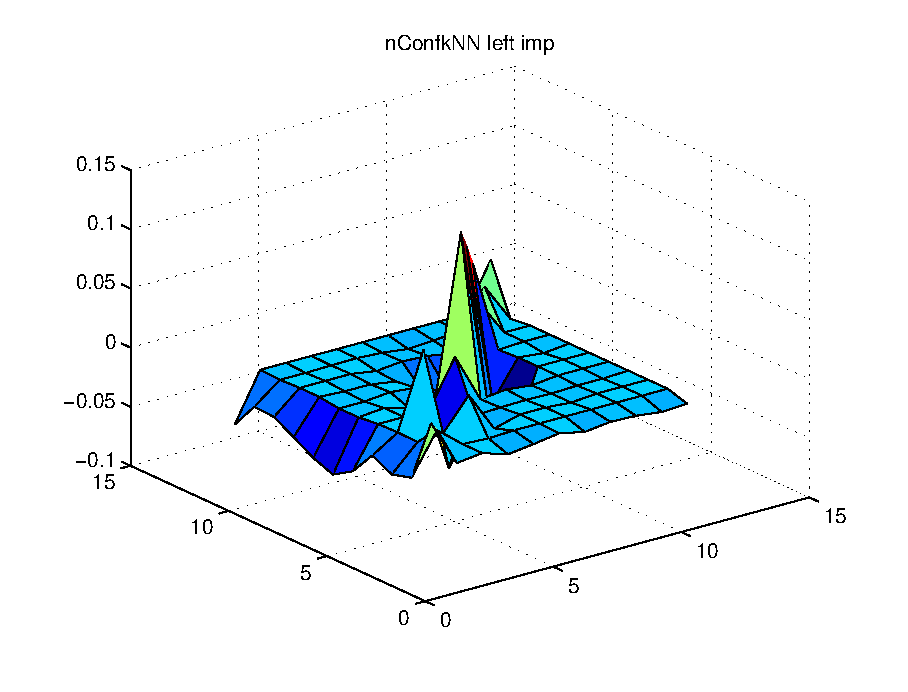
\includegraphics[scale=0.4]{./matlab_output/nConfkNN_left_imp_LDA_2.eps}
  \caption{Visualization of the left-arm per-activity improvement by LDA as referenced in Equation~\ref{eq:left_LDA_Conf_Imp}.}
  \label{fig:conf_left_imp_surf}
\end{figure}

\begin{figure}
  \centering
  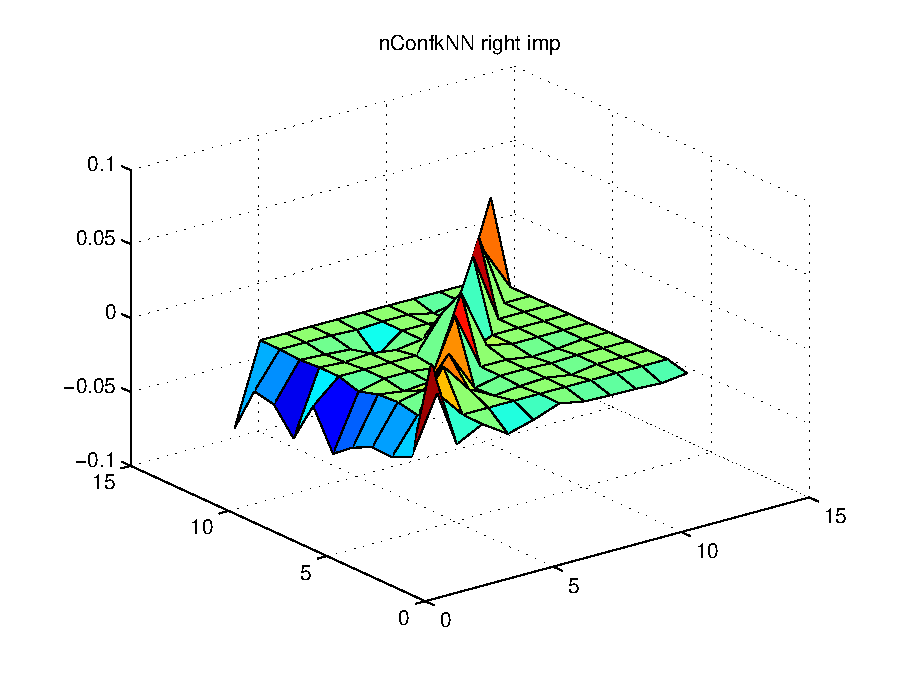
\includegraphics[scale=0.35]{./matlab_output/nConfkNN_right_imp_LDA_3.eps}
  \caption{Visualization of the right-arm per-activity improvement by LDA as referenced in Equation~\ref{eq:right_LDA_Conf_Imp}.}
  \label{fig:conf_right_imp_surf}
\end{figure}

\subsubsection{Improvement evaluation}
The diagonal values in the improvement visualization indicate an overall stronger true positive rate. Moreover the rest of the matrix containing the false positive rates of classification confusion are overall negative.  In particular we can observe that the null activity confusion is highly reducing with this data, which has effectively been exchanged into correct classifications.

However, if we focus on the activities which previously were found particularly difficult by the baseline classification the results are less impressive. Although slightly improved, both struggling pairs of open vs. close hood (49 and 50) and open vs. close left door (52 and 53) have received additional confusion.

Generally recording similar effect on both sets we use the left arm as an example. The true positive of open and close hood are here increased by 3.5\% and 1.9\%, while taking of 0.76\% and 0.41\% more confusion respectively. The toughest challenge of discriminating open and close left door have an increased true positive rate of 2.8\% and 0.66\%, for an additional confusion of 2.7\% and 3.9\%.

The feature extraction method thus increases the general performance, but does not improve the problematic activity discrimination and although introducing higher computational speed, the reduced number of features do not solve our initial issue with certain activity pairs.

\subsection{Performance by Increasing Data Amount}
The original dataset has been assembled sophisticatedly with the aim of satisfying the need for creating a working classification model with a minimum amount of measurements. By looking at the evolution of classification precision the study analyzes the compromise between performance and efficiency with the idea that less data induces higher computational speed.

\begin{figure}[t]
  \centering
  \includegraphics[scale=0.40]{./matlab_output/score_perc_left_3.eps}
  \caption{Evolution of classifier precision over percentage of data from 10\% to 100\% for left-arm dataset.}
  \label{fig:score_evo_left}
\end{figure}

\begin{figure}[t]
  \centering
  \includegraphics[scale=0.35]{./matlab_output/score_perc_right_3.eps}
  \caption{Evolution of classifier precision over percentage of data from 10\% to 100\% for right-arm dataset.}
  \label{fig:score_evo_right}
\end{figure}

While the original goal is to analyze which specific activities require more data to be classified, the evolution of the precision is although linear with the growing amount of data. The focus therefore shifted towards evaluating how the precision specifically grows over increasing the data amount which has been visualized for both datasets respectively in Figure~\ref{fig:score_evo_left} and Figure~\ref{fig:score_evo_right}. 

Although more conclusive results would preferably require more data as the original dataset has been delicately established by a certain amount of repetitions of each activity, the results still yield that the precision slowly saturates as we approach the full dataset.

Looking at the left-arm dataset, the precision already yields 84.39\% at only 10\% data, and reaches a full 91.4\%, only 0.6\% away from the maximum precision, at 80\% data. We can finally observe it flattening completely out as of 90\% data at maximum performance.

Similarly the right-arm dataset lands a 82.14\% precision at 10\% data which increases all the way to 89.56\% for 60\% data and finally achieves next to full performance at 80\% with a 90.54\% precision.

The final results depicted in Table~\ref{tab:evo_prec} tells of a performance saturation, that finally indicates that the precision will not be much further increased by performing more measures and will not solve the problem of per-activity performance issues regarding both pair-wise classification and general performance.

\begin{table}[t]
\centering
\caption{Precision evolution over amounts of data.}
\begin{tabular}{|l|l|l|}
\hline
           					&\textbf{Left arm baseline} 	&\textbf{Right arm baseline}		\\ \hline
\textbf{10\%}  				& 84.39\% 		 				& 82.14\%							\\ \hline
\textbf{60\%} 				& 90.83\%		 				& 89.56\%							\\ \hline
\textbf{80\%}  				& 91.4\%		 				& 90.54\%							\\ \hline
\textbf{100\%}  			& 92.04\% 		 				& 90.95\%							\\ \hline

\end{tabular}
\label{tab:evo_prec}
\end{table}

%=====================================================================

\section{Results}
Through the exploration of different improvement methods for the original baseline we can assemble a summarizing overview expanded in Table~\ref{tab:results}.

The final results justifies feature selection as the most effective improvement of the ones studied.

\begin{table*}[bp]
\centering
\caption{Comparable overview of explored improvement schemes}
\begin{tabular}{|l|l|l|l|l|l|}
\hline
           							&\textbf{Left arm} 			&\textbf{Left arm LDA}		&\textbf{Right arm}		&\textbf{Right arm LDA}		&\textbf{Combined data}	\\ \hline
\textbf{Precision}  				& 92.04\% 		 			& 95.33\%					& 90.95\%				& 94.53\%					& 94.17\%				\\ \hline
\textbf{Error rate} 				& 7.96\%		 			& 4.67\%					& 9.05\%				& 5.47\%					& 5.83\%				\\ \hline
\textbf{$F_{1}$ score}  			& 92.03\%		 			& 94.8\%					& 90.40\%				& 93.80\%					& 93.55\%			\\ \hline
\end{tabular}
\label{tab:results}
\end{table*}

%=====================================================================

\section{Conclusions}
In a first time the study recognizes that the baseline classification of each dataset with minimum features and preprocessing yields relatively strong results. Both datasets producing $F_1 score$s of over 90\% tells us that the activity recognition for this quite reduced data set of 10 specific activities is of quite high standard initially.

Studying various ways of improving the per-activity and general classification performance we see that feature selection strikes as the most effective, as it reduces the size of the dataset by features and generally achieves a higher performance.

However, activities that are very similar as open and closing a door are particularly difficult to solve, not having been solved sufficiently with any of the proposed improvement schemes. Although one approach could be to combine all the explored solutions, unfortunately as none of them addresses the issue specifically the problem is prone to overlap and remain improved, but not solved in a real-world application. 

Several approaches can be taken towards this per-activity issue. Should one although seek to solve the issue properly an option would be to introduce sensor weights. Through this approach one could perhaps handle the issue with only certain sensor registering the difference in impact of quite similar tasks.

Specificity comes at a cost, and a compromise between activity specificity and classification performance must be addressed when developing the set of classes to be recognized. By example, a possible option to solve the issue with opening and closing left car door would be to merge the activities into operating left car door, and such merging the classes with their features, which would effectively solve the problem.

%=====================================================================

\section{Future work}
An interesting possibility for further addressing the issue with specificity would be to evaluate both methods proposed in the conclusion. Evaluating different sensor weighting options as well as reducing the specificity would effectively be a next step in evaluating how we can approach more successfully specific \textit{Human Activity Recognition} applications.

%=====================================================================

%\begin{figure}
%\centering
%\epsfig{file=fly.eps}
%\caption{A sample black and white graphic (.eps format).}
%\end{figure}

%\begin{figure}[t]
%\begin{center}
%\fbox{\rule{0pt}{2in}
%   \includegraphics[width=0.3\linewidth]{WorkFlow.png}}
%\end{center}
%   \caption{A workflow diagram of our pipeline.}
%\label{fig:long}
%\label{fig:onecol}
%\end{figure}

% Two columns
%\begin{figure*}
%\centering
%\epsfig{file=flies.eps}
%\caption{A sample black and white graphic (.eps format)
%that needs to span two columns of text.}
%\end{figure*}

% Dual-column table
%\begin{table*}
%\centering
%\caption{Some Typical Commands}
%\begin{tabular}{|c|c|l|} \hline
%Command&A Number&Comments\\ \hline
%\texttt{{\char'134}alignauthor} & 100& Author alignment\\ \hline
%\texttt{{\char'134}numberofauthors}& 200& Author enumeration\\ \hline
%\texttt{{\char'134}table}& 300 & For tables\\ \hline
%\texttt{{\char'134}table*}& 400& For wider tables\\ \hline\end{tabular}
%\end{table*}
% end the environment with {table*}, NOTE not {table}!

%\begin{verbatim}
%{
%    "average_stars": 3.65,
%    "name": "Lene",
%    "review_count": 214,
%    "user_id": "WvhiRlcy-XYwiCof"
%}
%\end{verbatim}
\begin{figure*}[bp]
\centering
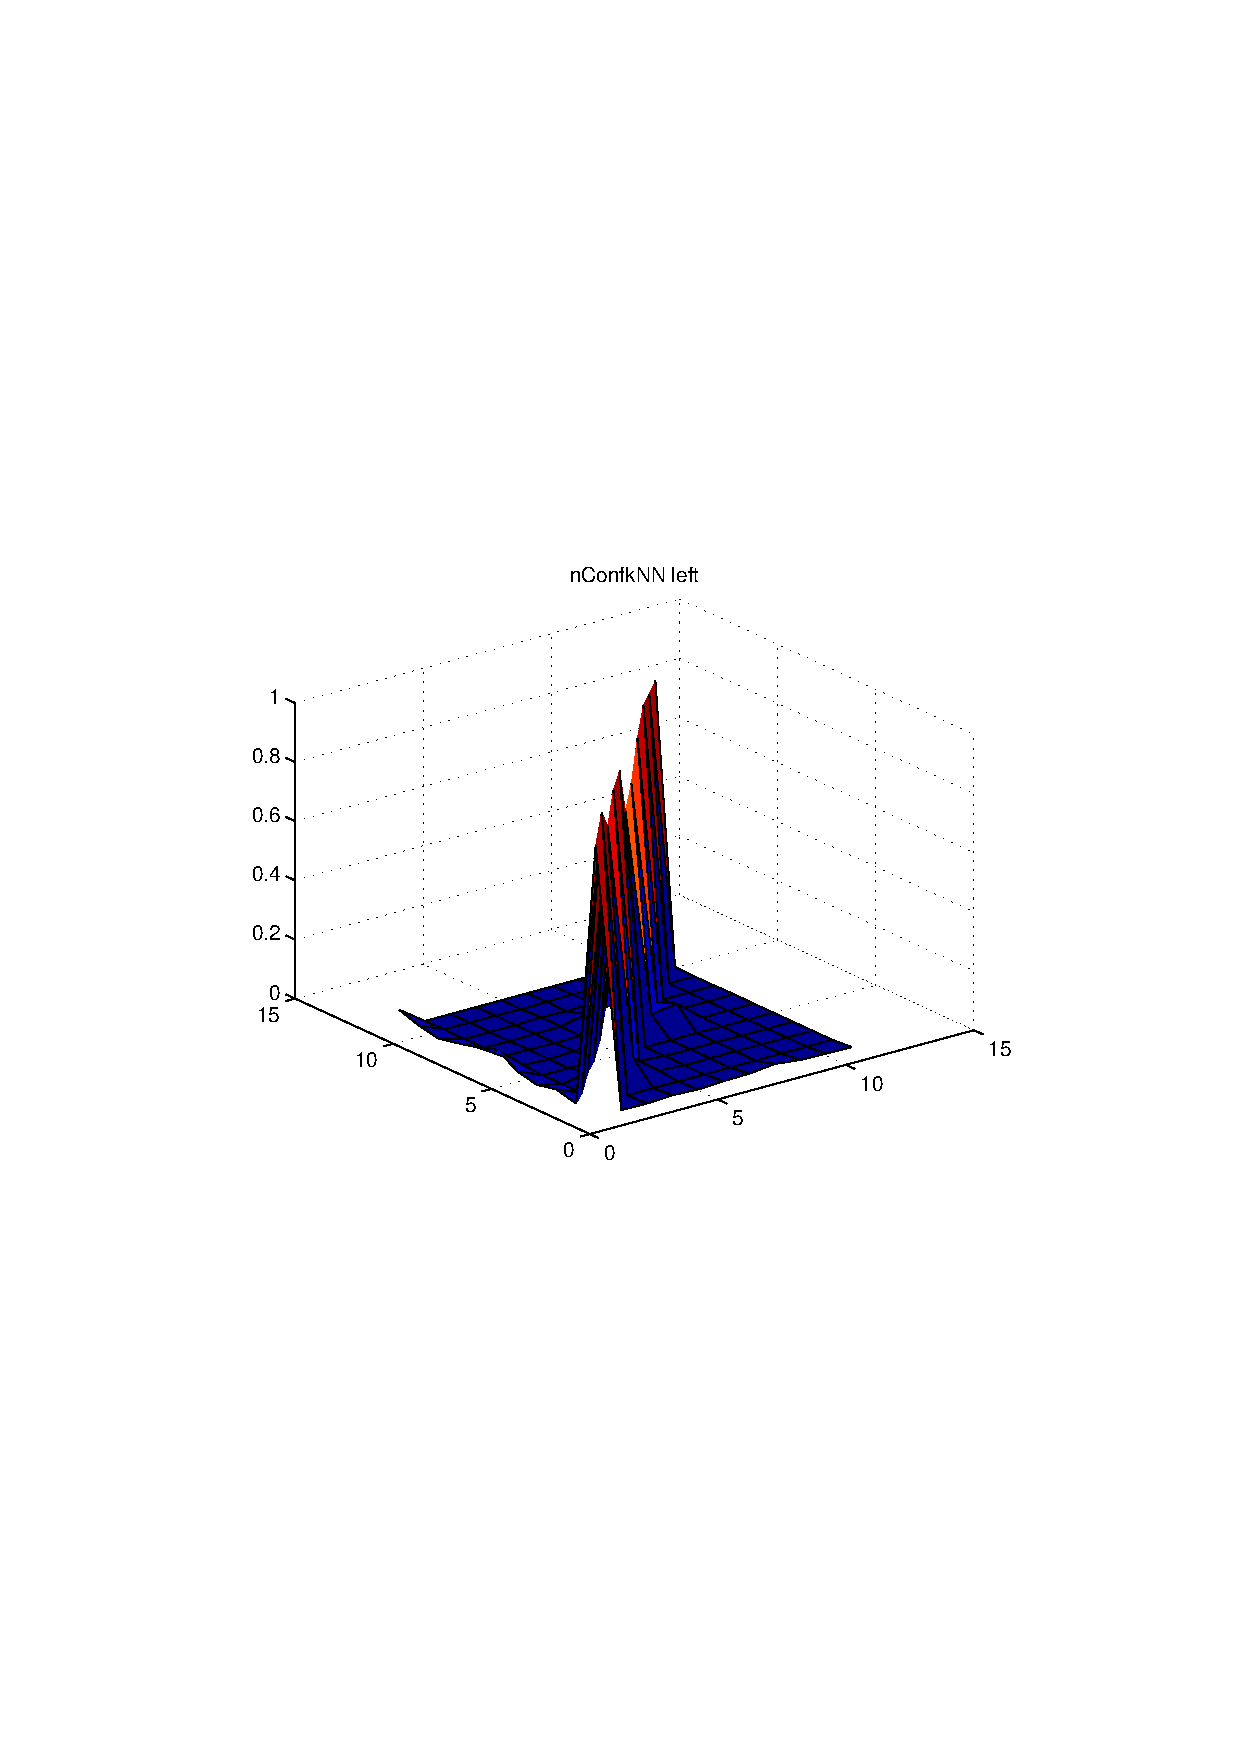
\includegraphics[width=1.0\linewidth]{visual_results/nConfkNN_left.jpg}
\caption{Confusion matrix for left arm performance.}
\label{fig:conf_left}
\end{figure*}

\begin{figure*}[bp]
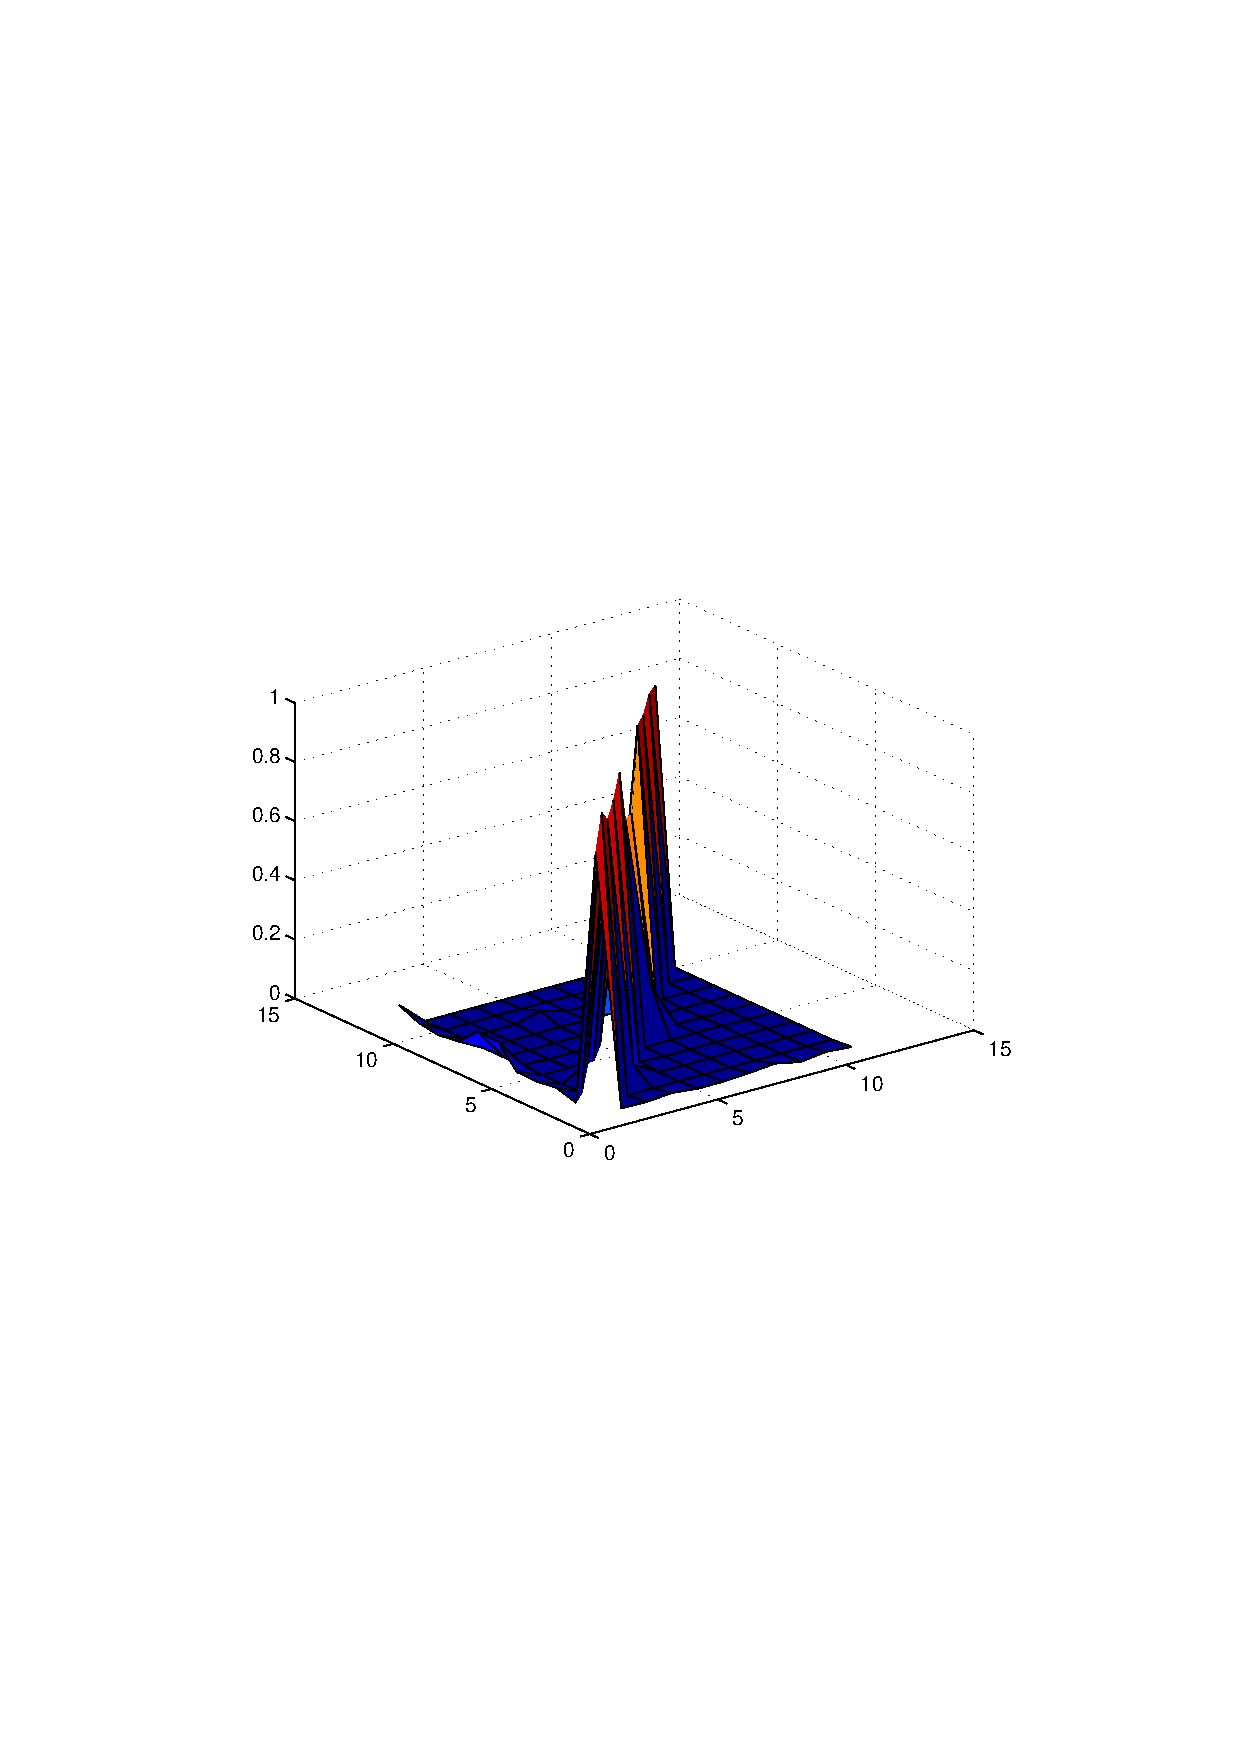
\includegraphics[width=1.0\linewidth]{visual_results/nConfkNN_right.jpg}
\centering
\caption{Confusion matrix for right arm performance.}
\label{fig:conf_right}
\end{figure*}

\begin{figure*}[bp]
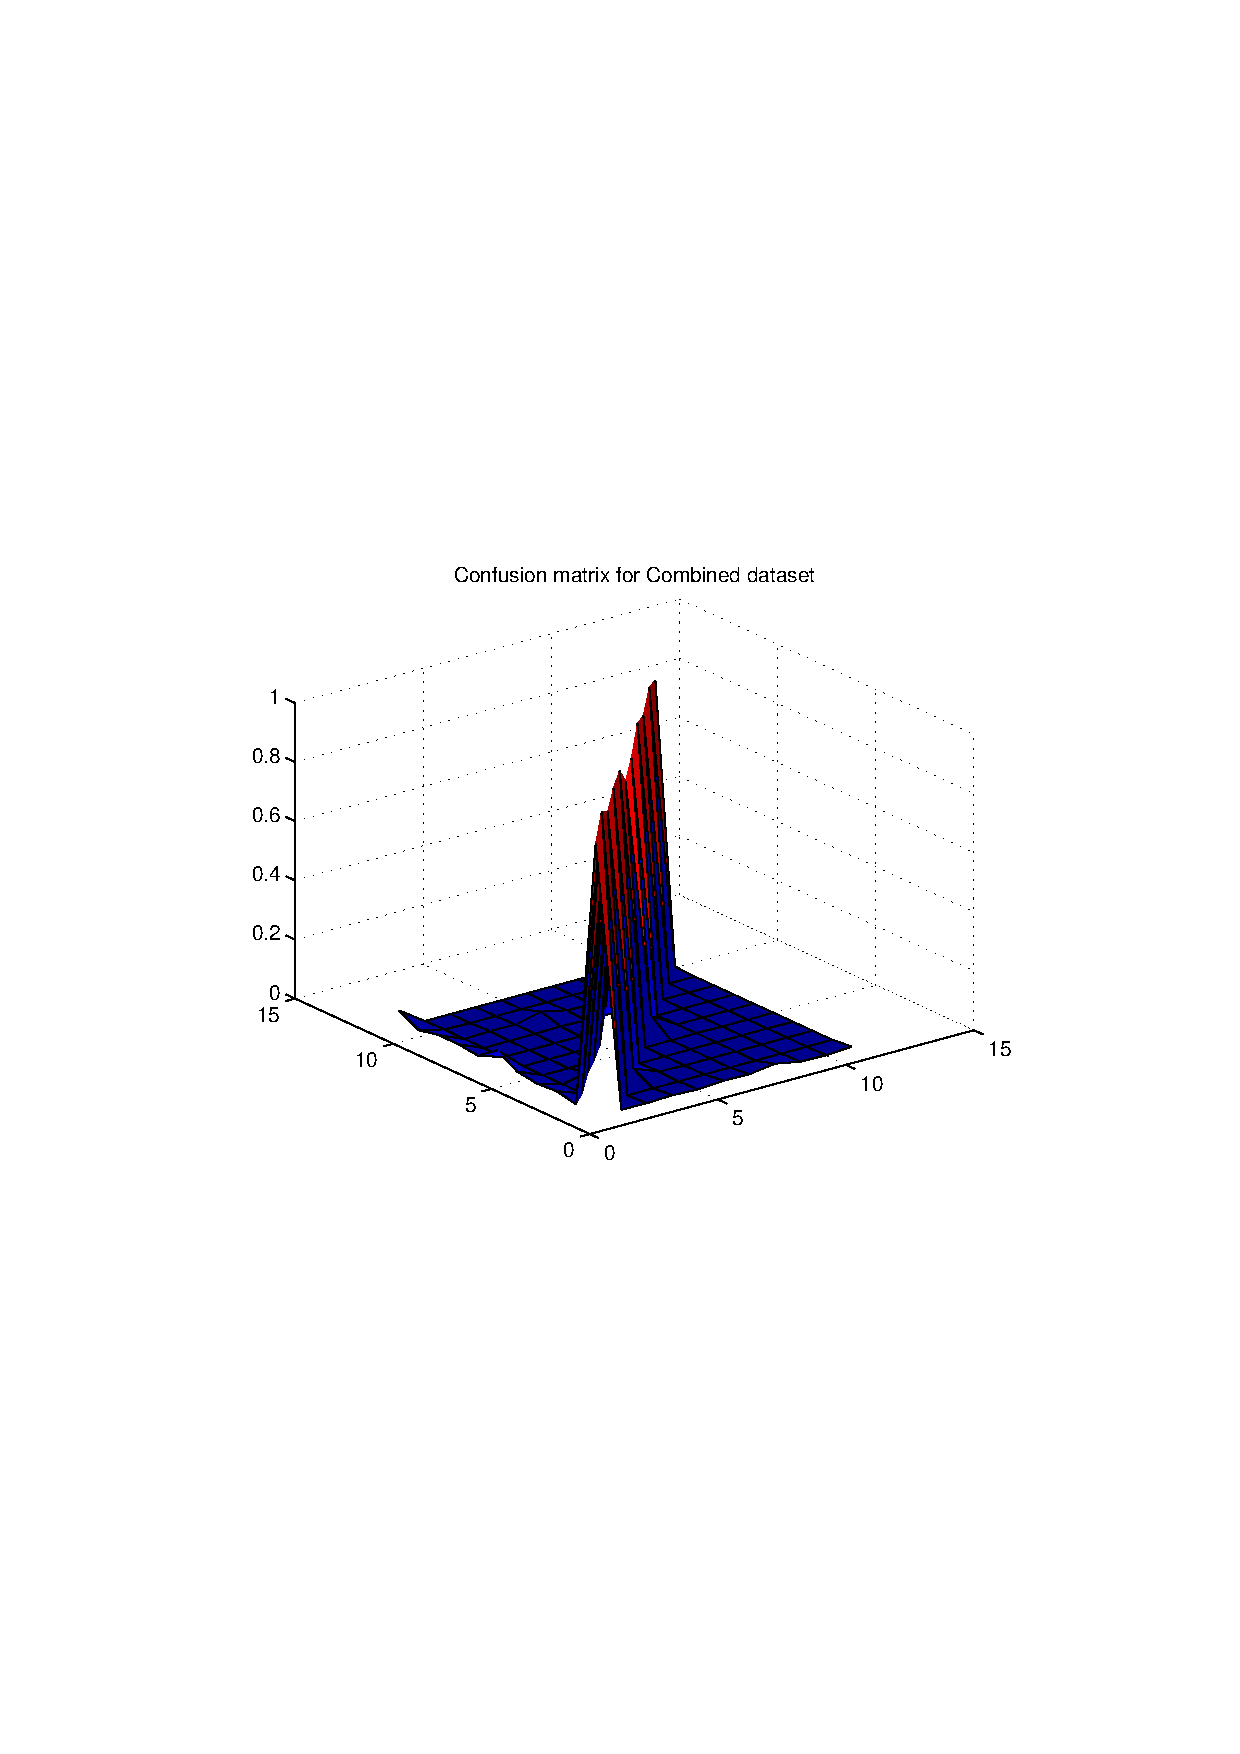
\includegraphics[width=1.0\linewidth]{visual_results/nConfkNN_both.jpg}
\centering
\caption{Confusion matrix for combined data performance.}
\label{fig:conf_both}
\vspace{150pt}
\end{figure*}
	
%=====================================================================

\begin{figure*}
\begin{center}
  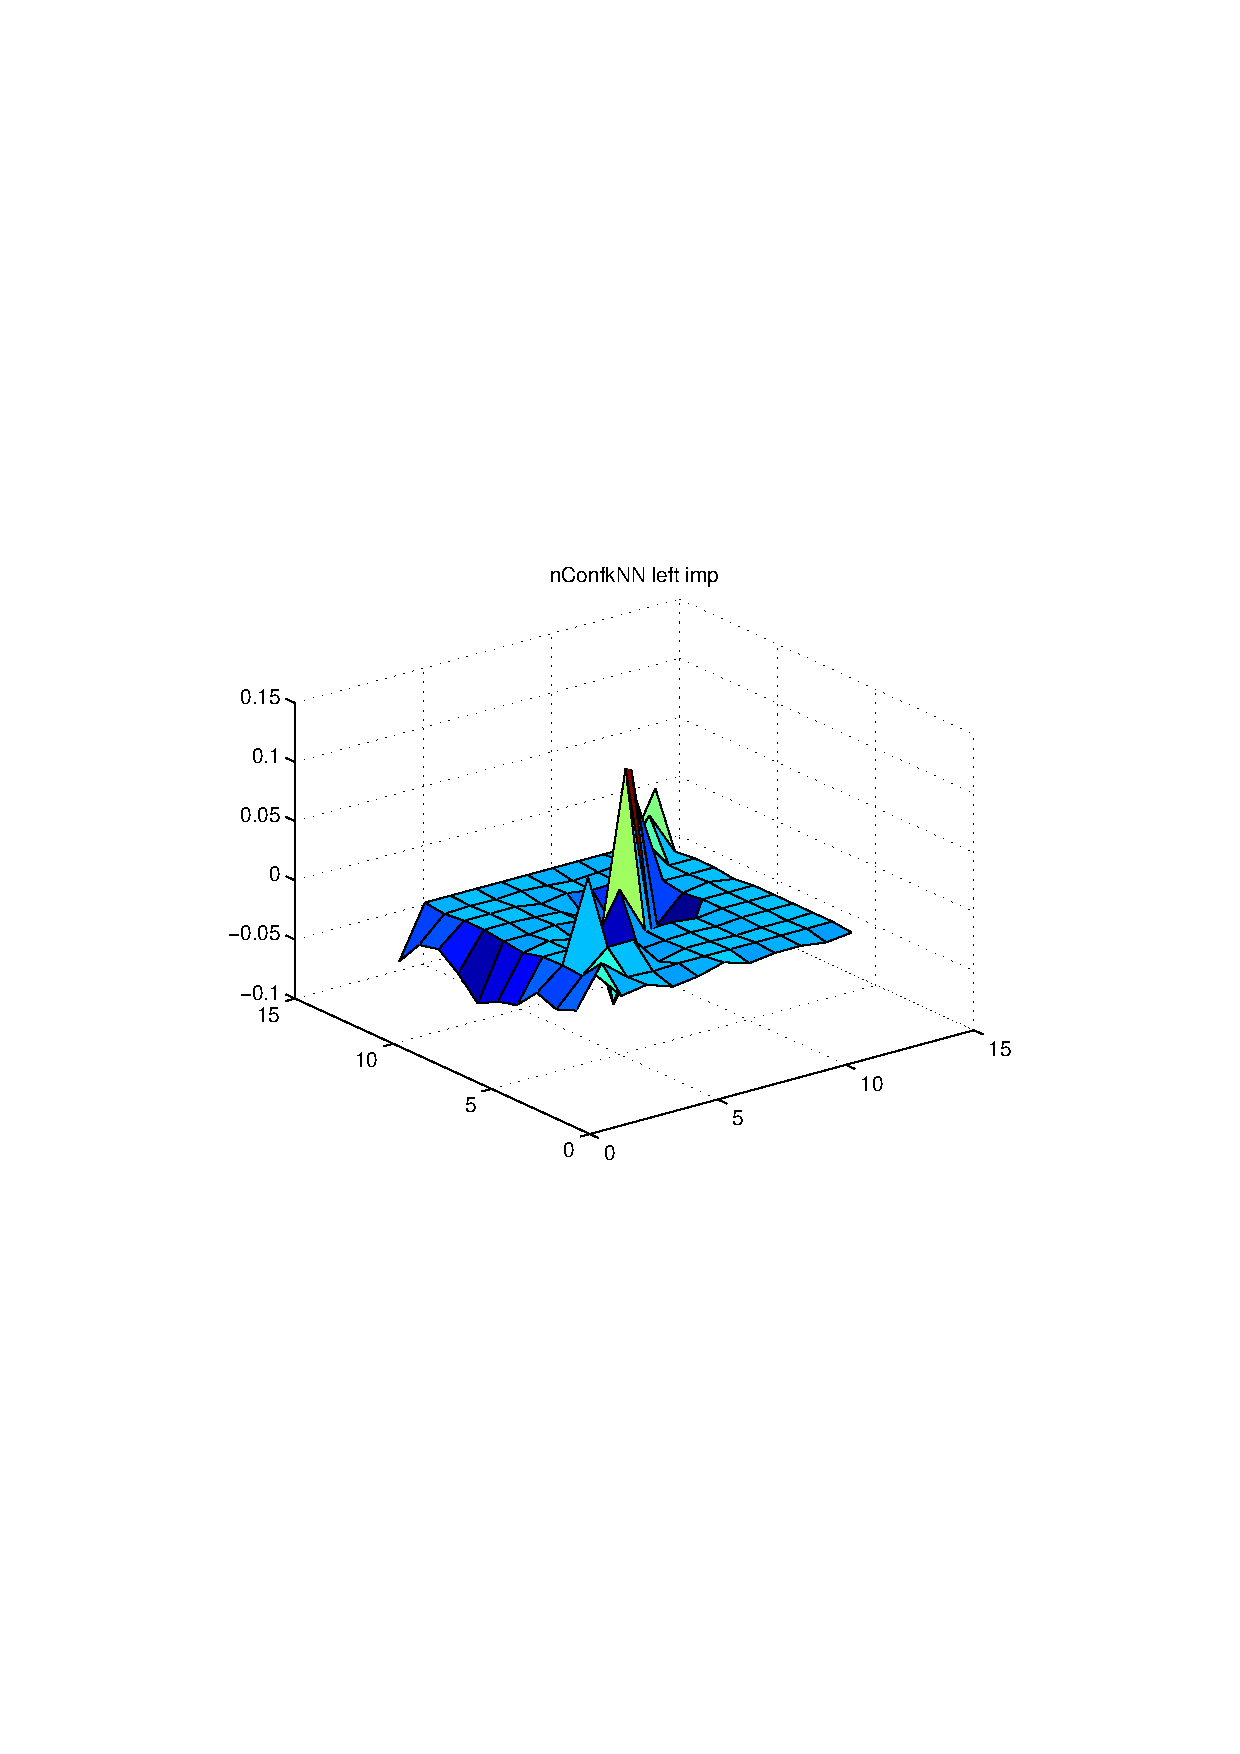
\includegraphics[width=1.0\linewidth]{visual_results/nConfkNN_left_imp_LDA.jpg}
\end{center}
  \caption{Breakdown of the left-arm per-activity improvement by LDA as referenced in Equation~\ref{eq:left_LDA_Conf_Imp}.}
  \label{fig:conf_left_imp_LDA}
\end{figure*}

\begin{figure*}
\begin{center}
  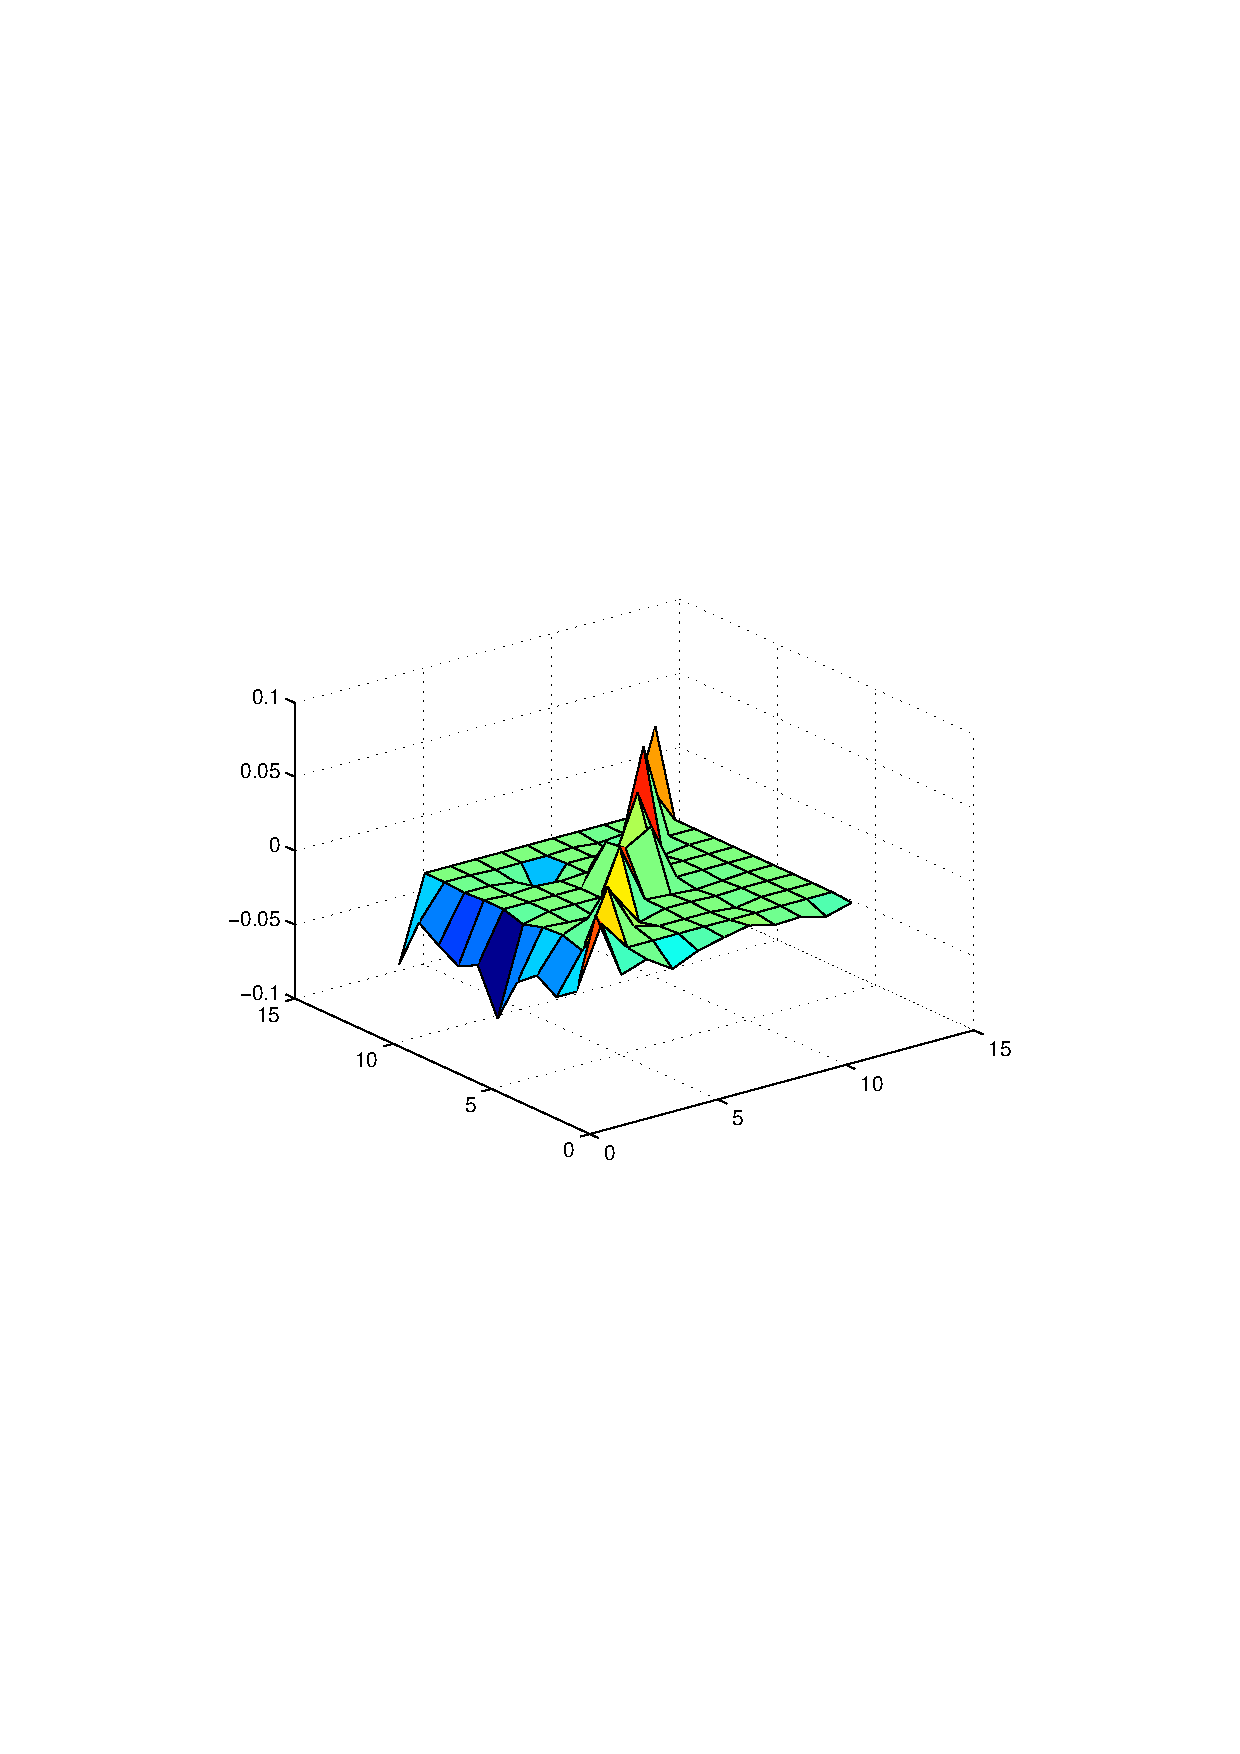
\includegraphics[width=1.0\linewidth]{visual_results/nConfkNN_right_imp_LDA.jpg}
\end{center}
  \caption{Breakdown of the right-arm per-activity improvement by LDA as referenced in Equation~\ref{eq:right_LDA_Conf_Imp}.}
  \label{fig:conf_right_imp_LDA}
\end{figure*}

%=====================================================================

%
% The following two commands are all you need in the
% initial runs of your .tex file to
% produce the bibliography for the citations in your paper.
\bibliographystyle{abbrv}
\bibliography{sigproc}
% add \cite{}'s for bilbiography. fill in sigproc.bib file

\end{document}
